\documentclass[10pt]{article}
\usepackage[UTF8]{ctex}

\usepackage[utf8]{inputenc} % allow utf-8 input
\usepackage{bm}
\usepackage{amsmath,amscd}
\usepackage{amssymb,array}
\usepackage{amsfonts,latexsym}
\usepackage{graphicx,subfig,wrapfig}
\usepackage{times}
\usepackage{psfrag,epsfig}
\usepackage{verbatim}
\usepackage{tabularx}
\usepackage[pagebackref=true,breaklinks=true,letterpaper=true,colorlinks,bookmarks=false]{hyperref}
\usepackage{cite}
\usepackage{algorithm}
\usepackage{multirow}
\usepackage{caption}
\usepackage{algorithmic}
\usepackage[amsmath,thmmarks]{ntheorem}
\usepackage{listings}
\usepackage{color}


\newtheorem{thm}{Theorem}
\newtheorem{mydef}{Definition}

\DeclareMathOperator*{\rank}{rank}
\DeclareMathOperator*{\trace}{trace}
\DeclareMathOperator*{\acos}{acos}
\DeclareMathOperator*{\argmax}{argmax}


\renewcommand{\algorithmicrequire}{ \textbf{Input:}}     
\renewcommand{\algorithmicensure}{ \textbf{Output:}}
\renewcommand{\mathbf}{\boldsymbol}
\newcommand{\mb}{\mathbf}
\newcommand{\matlab}[1]{\texttt{#1}}
\newcommand{\setname}[1]{\textsl{#1}}
\newcommand{\Ce}{\mathbb{C}}
\newcommand{\Ee}{\mathbb{E}}
\newcommand{\Ne}{\mathbb{N}}
\newcommand{\Se}{\mathbb{S}}
\newcommand{\norm}[2]{\left\| #1 \right\|_{#2}}

\newenvironment{mfunction}[1]{
	\noindent
	\tabularx{\linewidth}{>{\ttfamily}rX}
	\hline
	\multicolumn{2}{l}{\textbf{Function \matlab{#1}}}\\
	\hline
}{\\\endtabularx}

\newcommand{\parameters}{\multicolumn{2}{l}{\textbf{Parameters}}\\}

\newcommand{\fdescription}[1]{\multicolumn{2}{p{0.96\linewidth}}{
		
		\textbf{Description}
		
		#1}\\\hline}

\newcommand{\retvalues}{\multicolumn{2}{l}{\textbf{Returned values}}\\}
\def\0{\boldsymbol{0}}
\def\b{\boldsymbol{b}}
\def\bmu{\boldsymbol{\mu}}
\def\e{\boldsymbol{e}}
\def\u{\boldsymbol{u}}
\def\x{\boldsymbol{x}}
\def\v{\boldsymbol{v}}
\def\w{\boldsymbol{w}}
\def\N{\boldsymbol{N}}
\def\X{\boldsymbol{X}}
\def\Y{\boldsymbol{Y}}
\def\A{\boldsymbol{A}}
\def\B{\boldsymbol{B}}
\def\y{\boldsymbol{y}}
\def\cX{\mathcal{X}}
\def\transpose{\top} % Vector and Matrix Transpose

%\long\def\answer#1{{\bf ANSWER:} #1}
\long\def\answer#1{}
\newcommand{\myhat}{\widehat}
\long\def\comment#1{}
\newcommand{\eg}{{e.g.,~}}
\newcommand{\ea}{{et al.~}}
\newcommand{\ie}{{i.e.,~}}

\newcommand{\db}{{\boldsymbol{d}}}
\renewcommand{\Re}{{\mathbb{R}}}
\newcommand{\Pe}{{\mathbb{P}}}

\hyphenation{MATLAB}

\usepackage[margin=1in]{geometry}

\begin{document}
	
\title{	Numerical Optimization, 2020 Fall\\Homework 3}
\date{Due on 14:59 OCT 10, 2020\\
	请尽量使用提供的tex模板,单纯形法的表格可手绘拍照加入文档.
	}
\maketitle

%%%%%--------------------
\section{单纯形法}
以下均考虑非退化线性规划问题即可。
\begin{enumerate}
	\item[(i)] 考虑一线性规划问题的规范型如下:
	\begin{figure}[H]
		\centering
		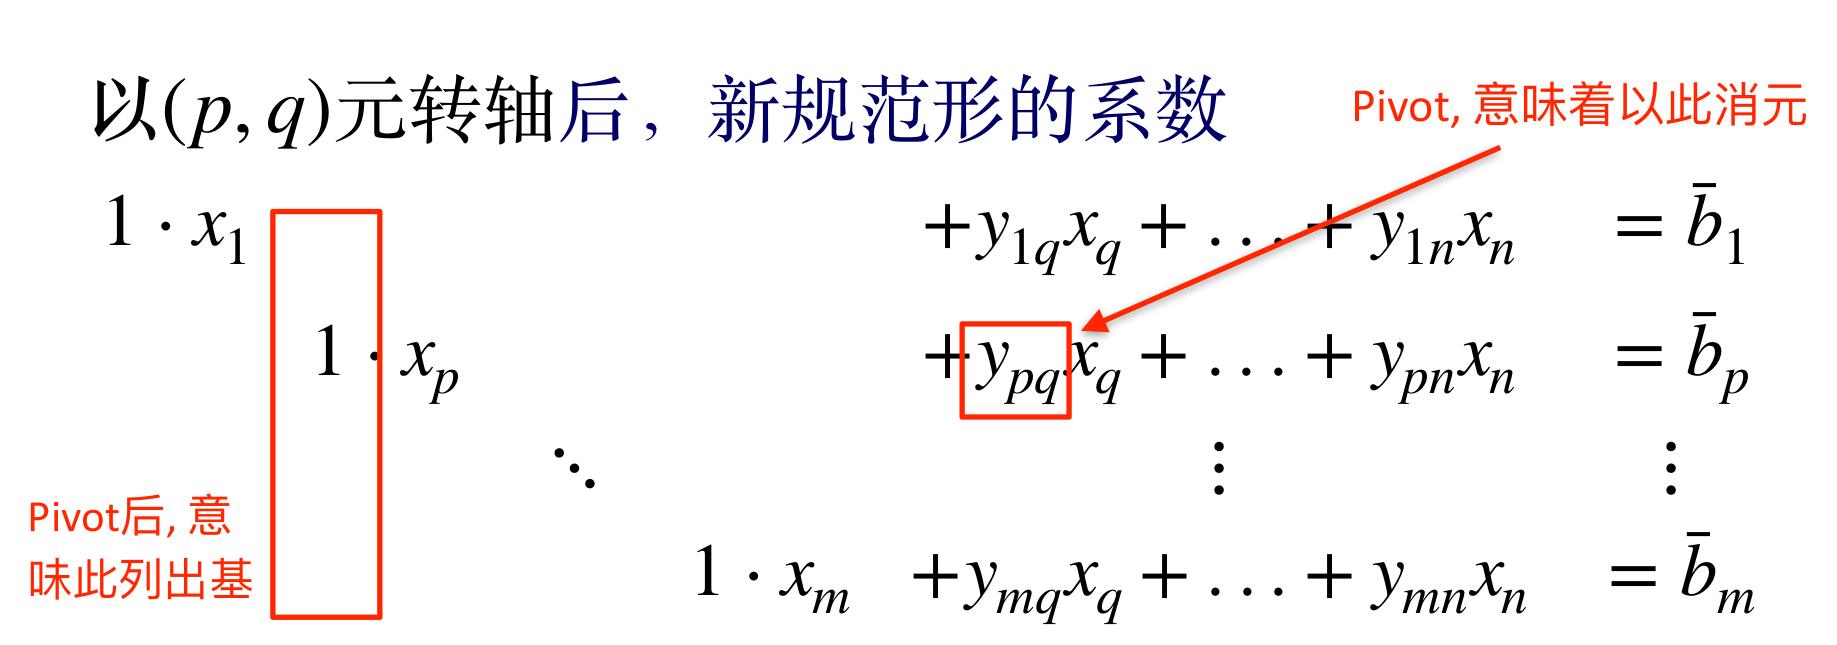
\includegraphics[width=0.55\linewidth]{hw3_1.png}
		%\caption{Accuracy demo.}
		\label{fig.prob1}
	\end{figure}
	记进基变量的下标为q, 转轴前分量j对应的reduced cost为$r_j$, 转轴后对应的reduced cost为$r'_j$。试证明reduced cost的更新公式为$r'_j=r_j - \frac{y_{pj}}{y_{pq}} r_q$(参考 Lecture 3中17页)。~\textcolor{red}{[20pts]}\\
	\textbf{解}\\
	\begin{align*}
	r_j'&=c_j-\hat{\lambda}^Ta_j \text{(By definition, where $a_j$ is the jth coloum of $N$)}\\	
	&=c_j-(\lambda^T+\frac{r_q}{y_{pq}}u_p)a_j \text{(By definition. $U_p$ is $p^{th}$ row of $B^{-1}$)}\\
	&=r_j - \frac{r_q}{y_{pq}}u_pa_j\\
	&=r_j-\frac{r_q}{y_{pq}}y_{pj}
	\end{align*}
	证毕。
	\item[(ii)] 单纯形表中右下角的-f对应当前基本可行解的目标函数值的相反数。试证明, 经过一次转轴后更新的-f对应更新后基本可行解对应的目标函数值的相反数 (参考 Lecture 3中20页)。~\textcolor{red}{[20pts]}
	\begin{figure}[H]
		\centering
		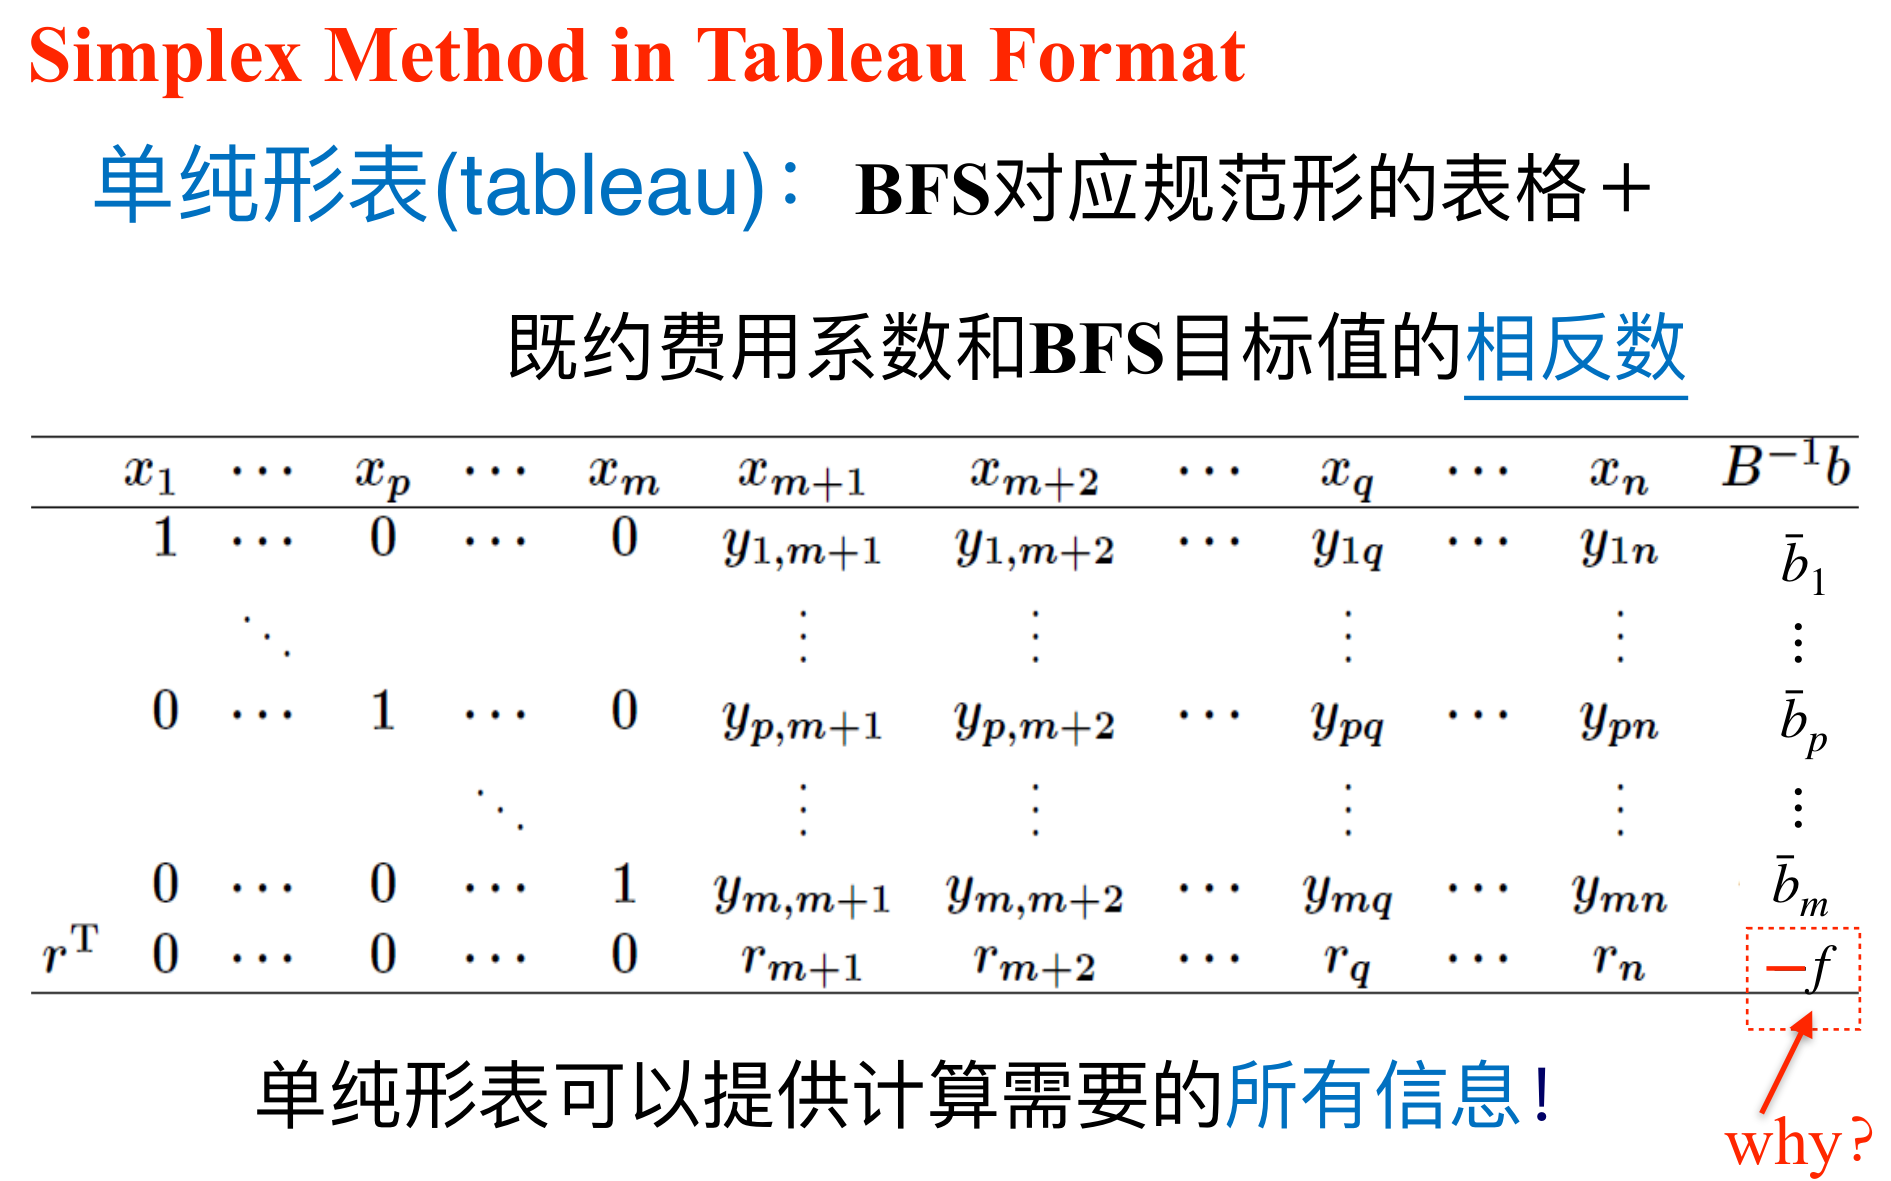
\includegraphics[width=0.55\linewidth]{hw3_2.png}
		%\caption{Accuracy demo.}
		\label{fig.prob2}
	\end{figure}
	\textbf{解}\\
	设$f'$为$-f$转轴更新后的值,$f\hat{f}$为更新后基本可行解对应的目标函数值得真实值,下证$f'=\hat{f}$。首先根据高斯消元的性质可得
	$$f' = f + \frac{r_q}{y_{pq}}\bar{b}_p$$
	根据目标函数的定义我们有
	\begin{align*}
	f&= \lambda^Tb\\
	\hat{f} &= \hat{\lambda}^Tb\\
	&=(\lambda^T+\frac{r_q}{y_{pq}}u_p)b\\
	&=\lambda^Tb + \frac{r_q}{y_{qp}}u_pb\\
	&=f + \frac{r_q}{y_{pq}}\bar{b_p} \,\,\text{(Since $U_p$ is $p^{th}$ row of $B^{-1}$, $u_pb=\bar{b}_p$)}\\
	&=f + \frac{r_q}{y_{pq}}\bar{b}_p
	\end{align*}
	即 $f'=\hat{f}$。因此经过一次转轴更新后的-f对应更新后基本可行解对应的目标函数值的相反数。
\end{enumerate}


\section{修正单纯形法}
\subsection{证明题}
试证明Lecture 4中20页$\lambda$的更新公式为: $\hat{\lambda}^T = \lambda^T + \frac{r_q}{y_{pq}} \bm{u}_p$。~\textcolor{red}{[20pts]}\\
\textbf{解}\\
首先我们定义初等矩阵$E_{pq}$,设$B(a_1,a_2,...,a_m)$,转轴元为$y_{pq}$,转轴后的基$\hat{B} = (a_1,...,a_{p-1},a_q,a_{p+1},...,a_m$
$$E_{pq} = [e_1,...,v,e_{p+1},...,e_m]$$
另定义$v$为
$$ v_i=\left\{
\begin{aligned}
-\frac{y_{iq}}{y_{p1}}, \text{ for $i\ne p$}\\
\frac{1}{y_{pq}},\text{ for $i=p$}
\end{aligned}
\right.
$$
则有$\hat{B}^{-1}=E_{pq}B^{-1}$.下面我们将$c_{\hat{B}},\hat{B}^{-1}$带入到$\hat{\lambda}$中
\begin{align*}
\hat{\lambda}^T &= (c_B+(0,...,0,-c_p+c_q,0,...,0))^TE_{pq}B^{-1}\\
&=C_B^TE_{pq}B^{-1}+(0,...,0,-c_p+c_q,0,...,0)^TB^{-1}\\
&=C_B^T(I-(\vec{0},\vec{0},..,e_p-v,...,\vec{0}))B^{-1} + (0,...,0,-c_p+c_q,0,...,0)^TB^{-1}\\
&=\lambda^T+(0,...,0,-c_p+c_B^Tv+(-c_p+c_q)v_p,0,...,0)^TB^{-1}\\
&=\lambda^T+(0,...,0,-c_p+c_1v_1+c_2+...+c_pv_p+...+c_mv_m-c_pv_p+c_qv_q)^TB^{-1}\\
&=\lambda^T + (0,...,0,-\frac{1}{y_{pq}}(c_1y_{1q}+...+c_my_{mq})+\frac{c_q}{y_{pq}},0,...,0)^TB^{-1}\\
&=\lambda^T + (0,...,0,\frac{c_q-z_q}{y_{pq}},...,0)^TB^{-1}\\
&=\lambda^T + \frac{r_q}{y_{pq}}u_p
\end{align*}
证毕。

\subsection{计算题}
试用两阶段法求解如下线性规划问题(详见Lecture 4第13页), 给出各个步骤的单纯形表。~\textcolor{red}{[40pts]}
\begin{figure}[H]
	\centering
	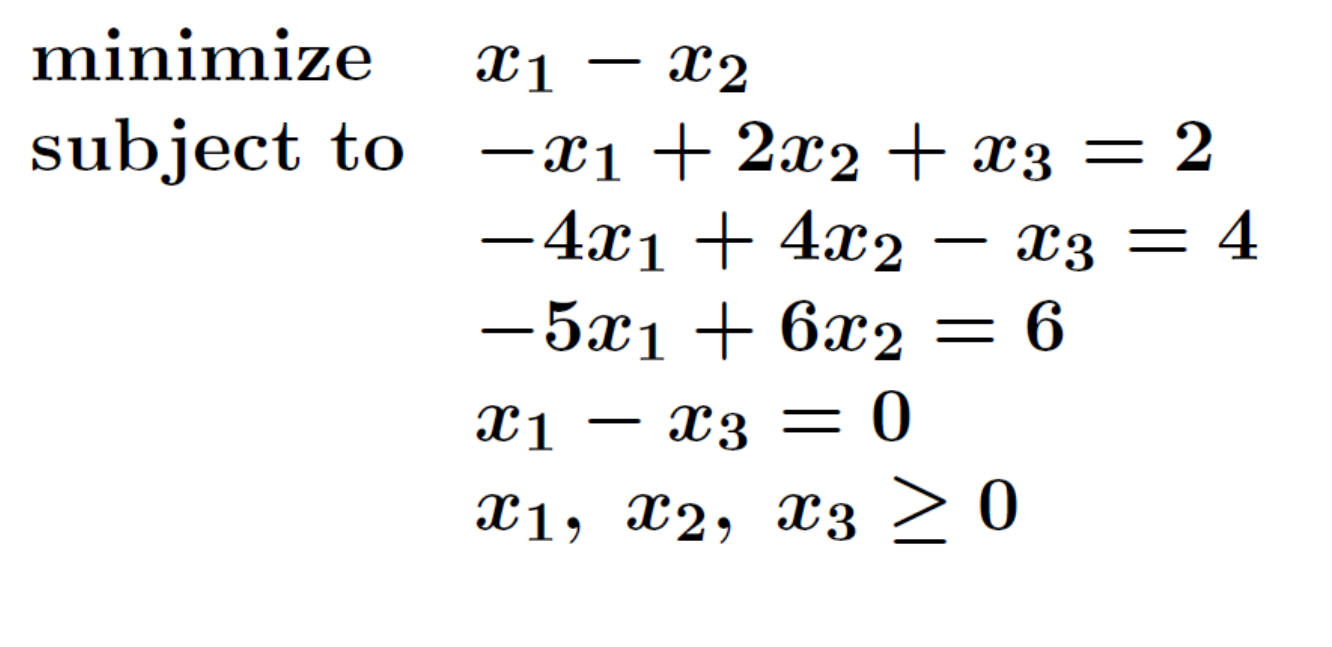
\includegraphics[width=0.4\linewidth]{hw3_3.png}
	%\caption{Accuracy demo.}
	\label{fig.prob3}
\end{figure}

\begin{figure}[H]
	\centering
	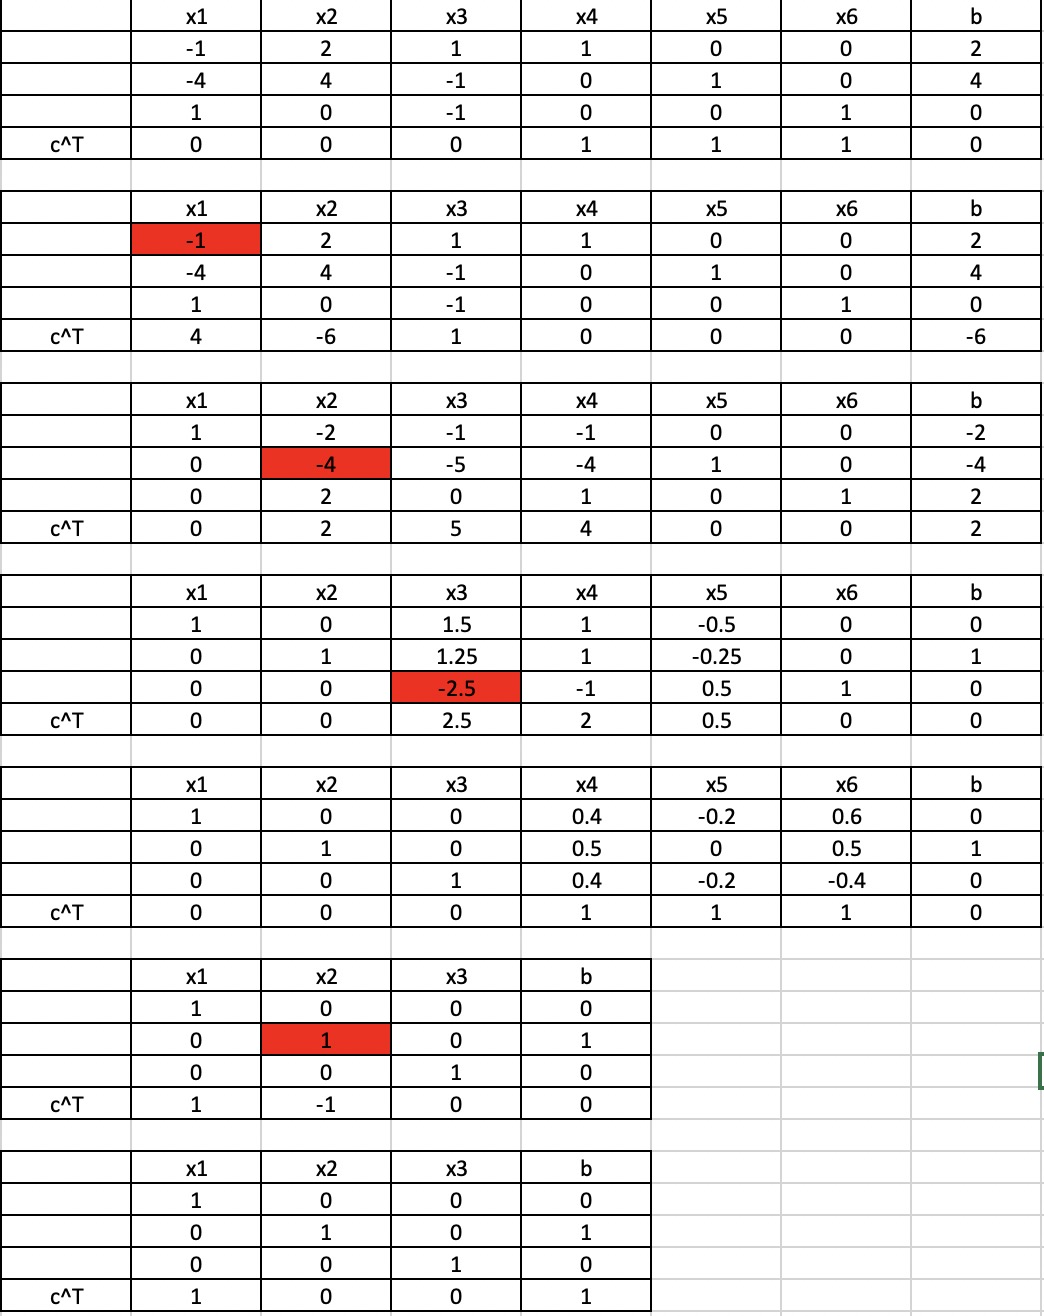
\includegraphics[width=0.4\linewidth]{table.png}
	%\caption{Accuracy demo.}
\end{figure}
于是我们有:$x_1=0,x_2=1,x_3,0$,并且最优值是$-1$。
\end{document} 